\documentclass{article}
\usepackage{graphicx}
\graphicspath{ {./} }
\usepackage{color}

\usepackage{amsmath}
\usepackage{commath}
\usepackage{amssymb}
\usepackage{listings}
\usepackage{algorithm2e}
\usepackage{float}

\usepackage{hyperref}
\hypersetup{linktoc=all}

\usepackage{listings}
\usepackage{geometry}
\geometry{margin=1in}
\usepackage{color}
\definecolor{light-gray}{gray}{0.95}
\lstset{numbers=right,
                basicstyle=\tiny,
                numberstyle=\tiny,
                breaklines=true,
                backgroundcolor=\color{light-gray},
                numbersep=5pt,
                xleftmargin=.5in,
                xrightmargin=.5in}

\sloppy
\definecolor{lightgray}{gray}{0.5}
\setlength{\parindent}{0pt}

\begin{document}

\title{Lab 5: JPEG Compression Fingerprints}
\author{Brian Hosler \& Sarah Peachey }
\maketitle


\section{Detecting JPEG Compression Using DCT Coefficients Quantization
Fingerprints}

\qquad JPEG compression leaves behind fingerprints in the image's DCT coefficients.
These fingerprints become clearly visible in the histogram of the DCT coefficients. This
is due to the blocking effects and quantization that takes place during the JPEG compression
process. The DCT coefficients histogram of a JPEG compressed image will not
be smooth, it will contain gaps and the width of the gaps corresponds to the
quantization level used during the JPEG process. If an image was doubly JPEG
compressed the bins in the histogram will be grouped by a different width,
so there new bins will either be zero or dramatically increase in height. 

    
    \begin{verbatim}
%Assignment 5
%Brian Hosler and Sarah Peachey
f1=imread('Assignment 5 - Part 1 Files/DCTfprints1.tif');
f2=imread('Assignment 5 - Part 1 Files/DCTfprints2.tif');
f3=imread('Assignment 5 - Part 1 Files/DCTfprints3.tif');
f4=imread('Assignment 5 - Part 1 Files/DCTfprints4.tif');
f5=imread('Assignment 5 - Part 1 Files/DCTfprints5.tif');

figure
subBandHist(f1,2,2)
%no JPEG

figure
subBandHist(f2,2,2)
%step size 10

figure
subBandHist(f3,2,2)
%step size 6

figure
subBandHist(f4,2,2)
%no JPEG

figure
subBandHist(f5,2,2)
%step size 10
\end{verbatim}

\newpage 

As seen in Figure \ref{DCT1} DCT1fprints1.tiff is clearly not JPEG
compressed as there are no fingerprints in the histogram. Whereas Figure \ref{DCT2}
shows the image was compressed with quantization levels of 10, and Figure \ref{DCT3}
shows that image was compressed with quantization levels of 6. Figure
\ref{DCT4} again appears to have no fingerprints of JPEG compression visible
in the histogram. Finally figure \ref{DCT5} seems to show that the image was
JPEG compressed with quantization levels of 10, but it also has magnitudes
much greater than all the other images, especially at zero. So one could
assume that at first a bin size of 5 or 2 was used to compress the image and
the image was then double compressed with a quantization level of 10. I think
it would be 5 or 2 first because those numbers both evenly divide 10 so
multiple of the first quantization bins would evenly fit into the second
quantization bins. Which would result in the drastic spikes that are seen in
Figure \ref{DCT5}. 

\begin{figure}[H]
\centering
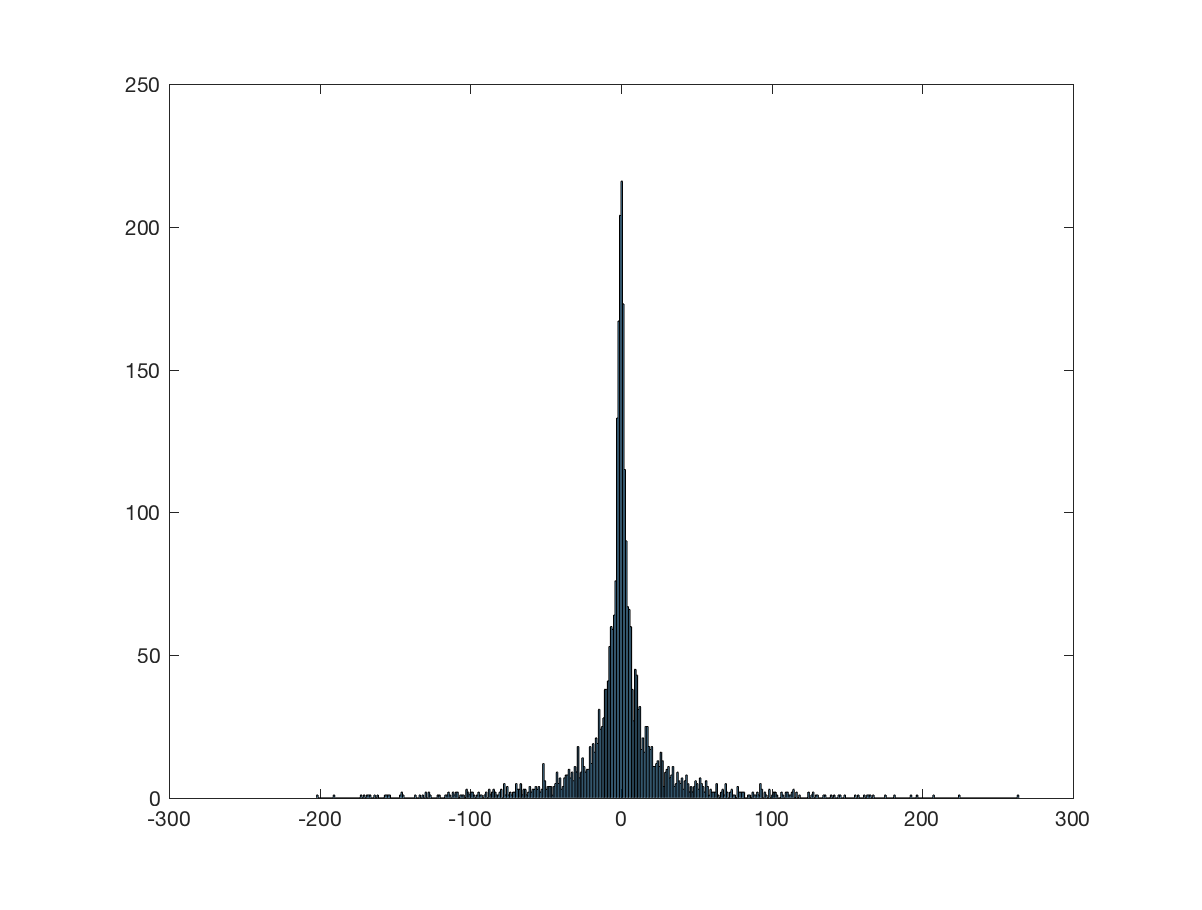
\includegraphics [width=3.5in]{lab5_01.eps}
\caption{The histogram of the DCT coeff's of DCTfprints1.tif}
\label{DCT1}
\end{figure}

\begin{figure}[H]
\centering
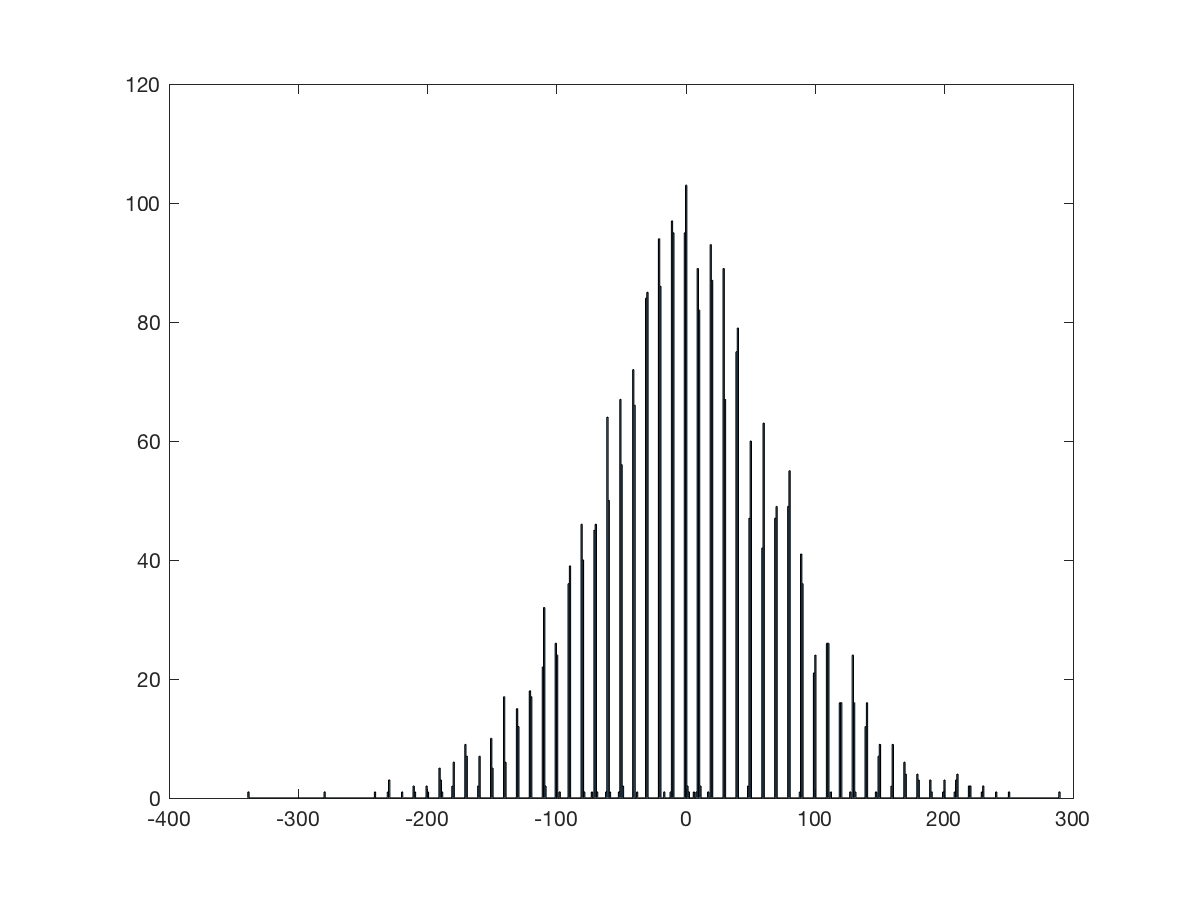
\includegraphics [width=3.5in]{lab5_02.eps}
\caption{The histogram of the DCT coeff's of DCTfprints2.tif}
\label{DCT2}
\end{figure}

\begin{figure}[H]
\centering
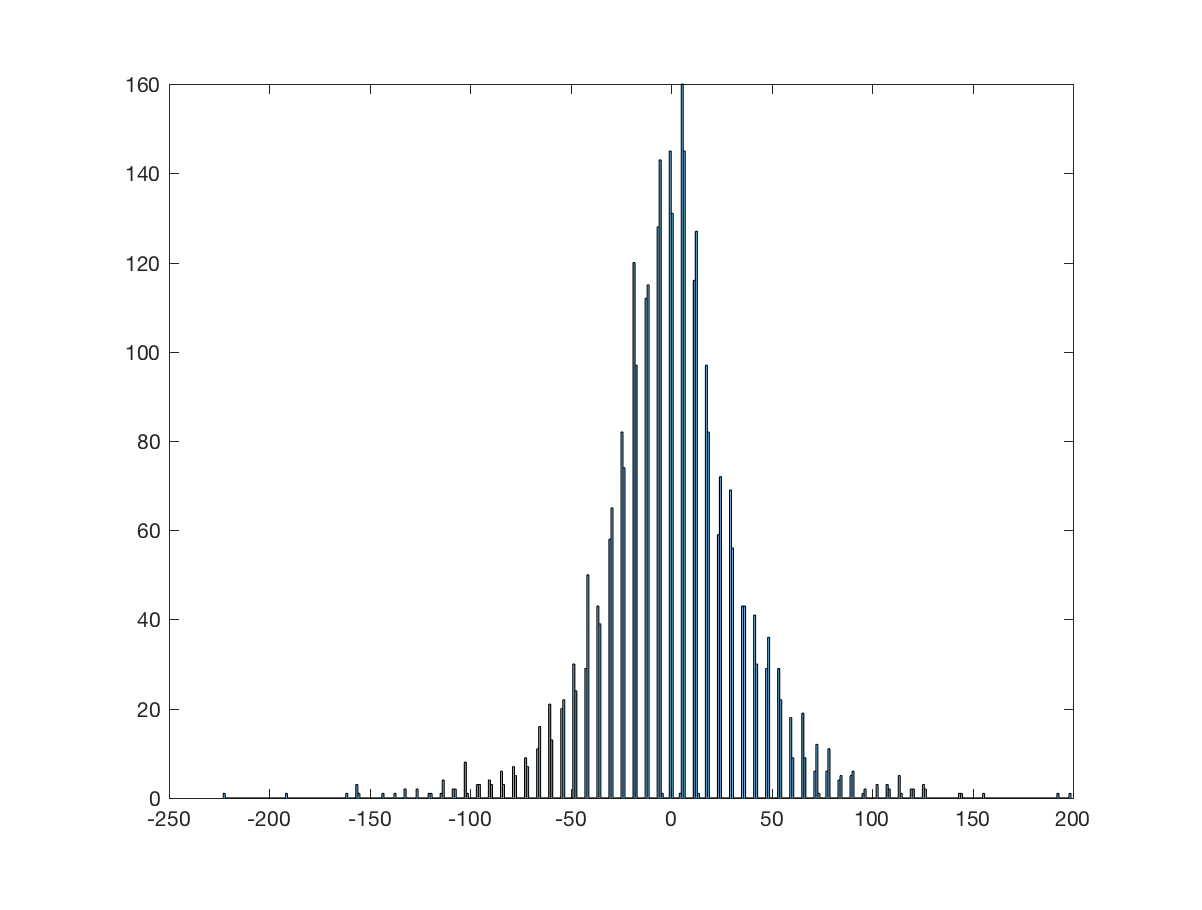
\includegraphics [width=3in]{lab5_03.eps}
\caption{The histogram of the DCT coeff's of DCTfprints3.tif}
\label{DCT3}
\end{figure}

\begin{figure}[H]
\centering
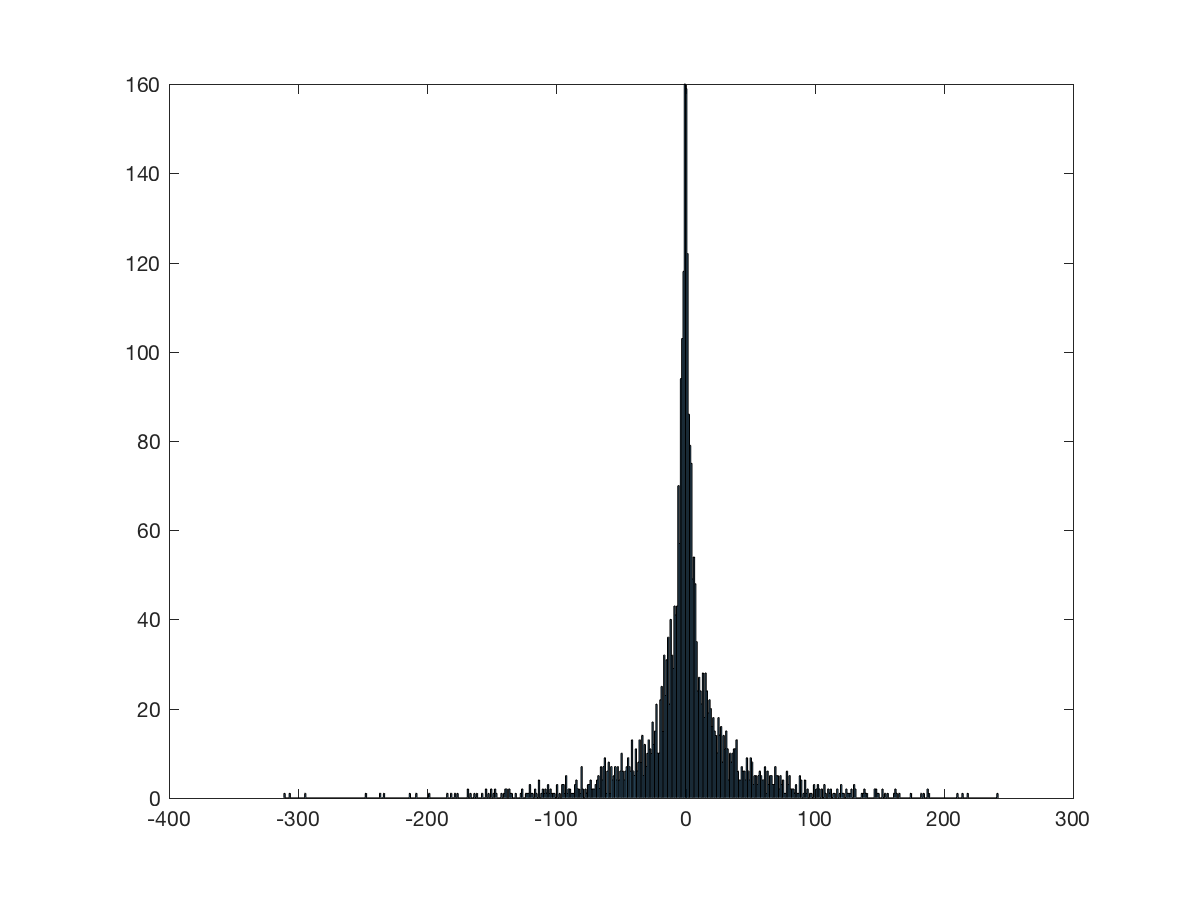
\includegraphics [width=3in]{lab5_04.eps}
\caption{The histogram of the DCT coeff's of DCTfprints4.tif}
\label{DCT4}
\end{figure}

\begin{figure}[H]
\centering
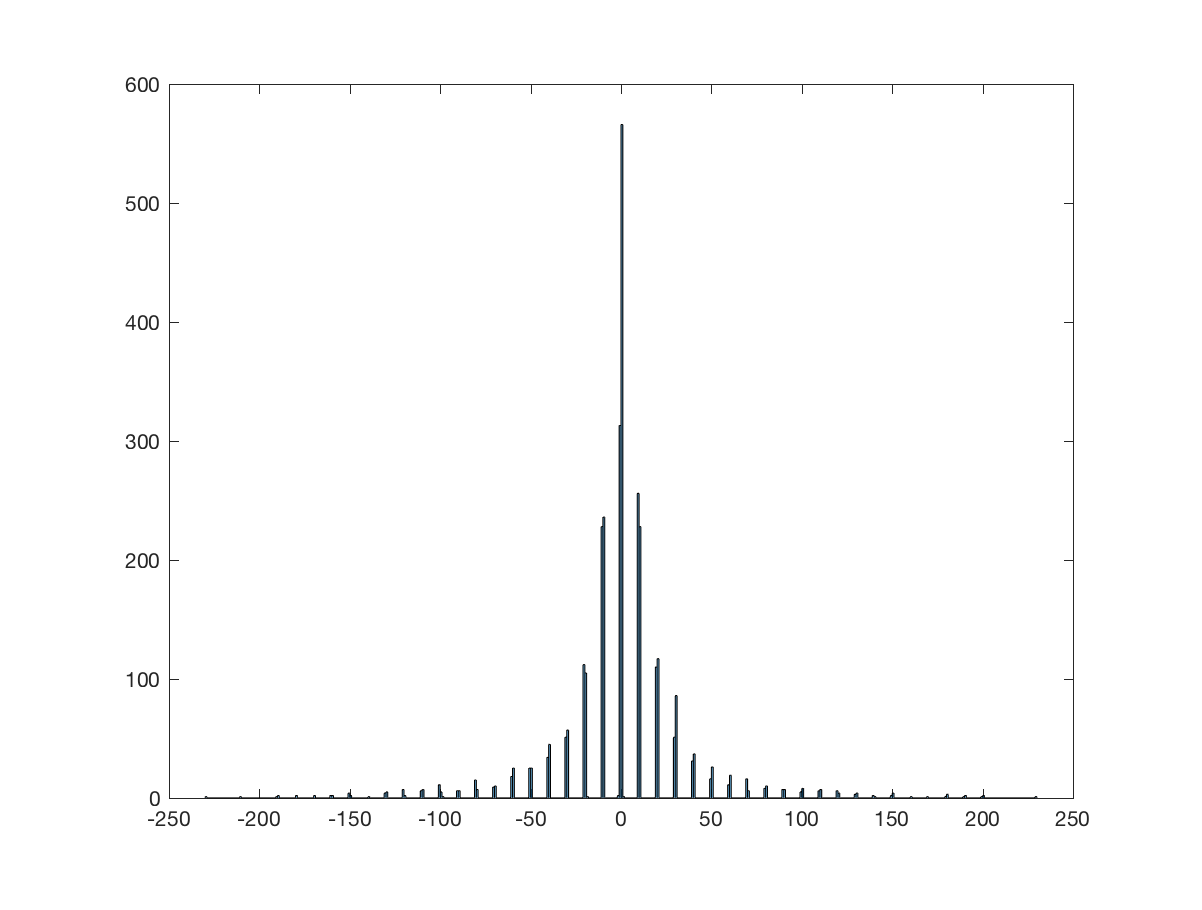
\includegraphics [width=3in]{lab5_05.eps}
\caption{The histogram of the DCT coeff's of DCTfprints5.tif}
\label{DCT5}
\end{figure}



\end{document}
    
